% a-project.tex, v-1.0.3 marcoreis baseado no
% abntex2-modelo-trabalho-academico.tex, v-1.9.7 laurocesar
% Copyright 2012-2018 by abnTeX2 group at http://www.abntex.net.br/ 
% 
% This work consists of the files ........
% 
% -----------------------------------------------------------------------------
% Modelo para desenvolvimento de documentação de projetos acadêmicos
% (tese de doutorado, dissertação de mestrado e trabalhos de monografias em geral) 
% em conformidade com ABNT NBR 14724:2011: Informação e documentação. 
% -----------------------------------------------------------------------------
% Opções para a documentação
%
% Fancy page headings 
%\documentclass[fancyheadings, subook]{Classes/a-prj}
%\documentclass[fancyheadings, sureport]{Classes/a-prj}
%
% Fancy chapters and sections headings 
%\documentclass[fancychapter, subook]{Classes/a-prj}
%\documentclass[fancychapter, sureport]{Classes/a-prj}
%
% Fancy page , chapters and sections headings
%\documentclass[fancyheadings, fancychapter, subook]{Classes/a-prj}
\documentclass[fancyheadings, fancychapter, sureport]{Classes/a-prj}
%
% -----------------------------------------------------------------------------
% Alguns comandos para a fancy page headings)
%
% Page header line width
%\footlinewidth{value}
%
% Page footer line width
%\headlinewidth{value}
%
% Page header and footer line width
%\headingslinewidth{value}
%
% Page header and footer lines without text
%\headingslinesonly
%
% The default line width is 0.3pt.
% Set the value to 0pt to remove the page header and/or footer line
%
% -------------------------------------------------------------------------------
% Formato de figuras suportado
% -------------------------------------------------------------------------------
% O formato das figuras depende da forma como o arquivo de saída é gerado.
% As figuras inseridas na pasta Figures serão automaticamente reconhecidas sem
% a necessidade de inserir a extensão do arquivo.
%
% O pdfLaTEX (PDF) suporta figuras com as extensões: pdf, jpg, png e mps.
%
% -------------------------------------------------------------------------------
% Árvore do diretório a-project.tex
%  Diretório
%       \Classes        (requerido)
%       \Figures        (requerido) --------------------------------->
%       \Figures\PDF    (optional)
%       \Figures\JPG    (optional) Figures located within these
%       \Figures\PNG    (optional) folders are searched automatically
%       \Figures\MPS    (optional)  by the a-prj class.
%       \Figures\EPS    (optional)
%       \Figures\PS     (optional) <--------------------------------
%       \Tables         (requerido)
%       \Others         (requerido)
%       \Chapters       (requerido)
%       \Appendices     (optional)
%       \References     (requerido)
%
% -------------------------------------------------------------------------------
% PDF File resumo
\ifpdf
    \hypersetup{
    	backref,
        colorlinks  = true,
        pdftitle    = Modelo de documentação,
        pdfauthor   = {Marco Reis, marco.a.reis@gmail.com},
        pdfsubject  = Mestre em Engenharia,
        pdfcreator  = Subtitulo,
        pdfproducer = PDFLatex,
        pdfkeywords = {documentação, latex, dissertação, tese}}
 \fi
%
% -------------------------------------------------------------------------------
% Relação de pacotes opcionais utilizados
\usepackage[utf8]{inputenc}
\usepackage[brazil]{babel}
\usepackage{longtable}
\usepackage{dcolumn}
\usepackage{multirow}
\usepackage{lscape}
%\usepackage{graphicx}
\usepackage{rotating}
%\usepackage{float,subfigure}
%\usepackage{graphicx, subfigure}
\usepackage{cite}
\usepackage[left=3cm,top=3cm,right=2cm,bottom=2cm]{geometry}
\usepackage[alf]{abntex2cite}
\usepackage{ifpdf}
\usepackage{shadow}
\usepackage{wrapfig}
\usepackage[normalem]{ulem}
\usepackage{makeidx}
\usepackage{yfonts}
\usepackage{algorithm}
\usepackage{algorithmic}
\usepackage{lmodern}
\usepackage[T1]{fontenc}
\usepackage{indentfirst}
\usepackage{color}
\usepackage{microtype}
\usepackage{lipsum}
\usepackage{caption}
\usepackage{subcaption}
%
\makeindex 
\setlength{\LTcapwidth}{\textwidth}
%
\newtheorem{theorem}{Teorema}
\newtheorem{definition}[theorem]{Definição}
%
% -------------------------------------------------------------------------------
% Configurações do pacote backref
\renewcommand{\backrefpagesname}{Citado na(s) página(s):~}
% Texto padrão antes do número das páginas
\renewcommand{\backref}{}
% Define os textos da citação
\renewcommand*{\backrefalt}[4]{
	\ifcase #1 %
		Nenhuma citação no texto.%
	\or
		Citado na página #2.%
	\else
		Citado #1 vezes nas páginas #2.%
	\fi
}
% 
% -------------------------------------------------------------------------------
% Início do documento raiz
\begin{document}
% Definição do título da página
    \university{Centro Universitário SENAI CIMATEC}
	%\faculty{Programa de...}
	%\school{Escola de...}
% 
    %\course{Engenharia Elétrica}
    \typework{Relatório dos desafios}
% 
	%\course{Mestrado em Modelagem Computacional e Tecnologia Industrial}
	%\typework{Disserta\c{c}\~ao de mestrado}
	%\typework{Exame de Qualificação de Mestrado}
% 
	%\course{Engenharia Elétrica}
	%\typework{Tese de doutorado}
	%\typework{Exame de Qualificação de doutorado}
%
% -------------------------------------------------------------------------------
% Informações gerais
    \thesistitle{Desafios: Webots, Turtlesim, Husky, CPP e Python}
    \hidevolume
    \thesisvolume{Volume 1 of 1}
    \thesisauthor{Marcella Giovanna Silva dos Santos}

    \thesisadvisor{Prof. Marco Reis, M.Eng.}
    %\hidecoadvisor
    %\thesiscoadvisor{Marco Reis}
    \thesisdegreetitle{Bacharel em Engenharia}
    \thesismonthyear{novembro 2021}
% 
    \maketitlepage
%
% ----------------------------------------------------------------------------
% Inserir Folha de rosto, Nota de estilo, folha de assinaturas, dedicatoria
    \begin{folharosto}

\begin{center}
\theauthor \\
%\theauthorrr \\
%\theauthorrrr \\
%\theauthorrrrr \\
\end{center}
\ \\
\ \\
\ \\
\ \\
\ \\
\begin{spacing}{2}
   \begin{center}
   {\LARGE {\bf \thetitle}}
   \end{center}
\end{spacing}
\ \\
\ \\
\ \\
\vspace*{85mm}
% \begin{flushright}

%    \begin{list}{}{
%       \setlength{\leftmargin}{7.5cm}
%       \setlength{\rightmargin}{0cm}
%       \setlength{\labelwidth}{0pt}
%       \setlength{\labelsep}{\leftmargin}}

%       \item \thetypework apresentada ao \thefaculty, Curso de \thecourse
%       do \theuniversity, como requisito parcial para a obten\c{c}\~ao do
%       t\'itulo de {\bf \thedegreetitle}.

%       \begin{list}{}{
%       \setlength{\leftmargin}{0cm}
%       \setlength{\rightmargin}{0cm}
%       \setlength{\labelwidth}{0pt}
%       \setlength{\labelsep}{\leftmargin}}

%       \item \'Area de conhecimento: Interdisciplinar

%       \item Orientador: \theadvisor
%       \newline \hspace*{2.1cm}  %{\it \theuniversity}

%       \end{list}
%    \end{list}

% \end{flushright}
\ \\
\ \\
\ \\
\ \\
%\begin{spacing}{1.5}
   \begin{center}
   Salvador \par
   \theuniversity \par
   2020
   \end{center}
%\end{spacing}

\end{folharosto}

    %\include{Others/NotaEstilo}
    %\include{Others/FolhaAssinaturas}
    %\include{Others/dedicatoria}
    %\include{Others/agradecimentos}
%
% ----------------------------------------------------------------------------
% Resumo/abstract, sumário e siglas
    \begin{romanpagenumbers}
        \begin{thesisresumo}
Com o intuito de aperfeiçoar e aprender alguns conceitos aplicados na robótica, foi realizados cinco desafios além de todos os tutoriais
de ros,os quais utilizam diferentes aplicações como: simulação de robôs, ROS, Webots e linguagens de programação (python e c++). Para que
dessa forma seja possivel a atuação no laboratório.
\ \\

%//todo realizar 

% use de três a cinco palavras-chave

\textbf{Palavras-chave}: Conceitos, robótica, simulação, ROS, programação.

\end{thesisresumo}

        \begin{thesisabastract}
In order to improve and learn some basic concepts in robotics, five challenges were carried out in addition to all the tutorials
of ros, they use different applications such as: training simulation, ROS, Webots and programming languages(python and c ++). For what
in this way it is possible to work in the laboratory
\ \\

% use de tr�s a cinco palavras-chave

\textbf{Keywords}: Concepts, robotics, simulation, ROS, programming.

\end{thesisabastract}

        % Make list of contents, tables and figures
        %\thesiscontents
        %Include other required section
        %\include{Others/abbreviation}
        %\include{Others/simbolos}
        %Switch the page numbering back to the default format
    \end{romanpagenumbers}
%
% ---------------------------------------------------------------------------
% Include thesis chapters
    \parskip=\baselineskip
    \chapter{Introdução}
\label{chap:intro}
\subsection{Webots}
Webots é um aplicativo de desktop de código aberto e multiplataforma usado para simular robôs. 
Ele fornece um ambiente de desenvolvimento completo para modelar, programar e simular robôs.
Ele foi projetado para um uso profissional e é amplamente utilizado na indústria, educação e pesquisa.
Cyberbotics Ltd. mantém Webots como seu produto principal continuamente desde 1998.\cite{Cyberbotics}
\subsection{Turtlesim SETPOINT POSITION }
Uma maneira simples de aprender o básico do ROS é usando o simulador turtlesim, que consiste na simulação 
de uma janela gráfica que mostra um robô com formato de tartaruga. Esta tartaruga pode ser movida por 
toda a janela utilizando comandos do ROS como roscore, rosrum... ou utilizando o teclado/joystick.\cite{ROSRoboticsByExample}
\subsection{Husky}
Husky é uma plataforma de desenvolvimento de robôs de médio porte. Sua grande capacidade de carga útil e sistemas de energia acomodam uma ampla variedade de cargas úteis, personalizadas para atender às necessidades de pesquisa. Câmeras estéreo, LIDAR, GPS, IMUs, manipuladores e muito mais podem ser adicionados ao UGV por nossos especialistas em integração. A construção robusta e o trem de força de alto torque do Husky podem levar sua pesquisa aonde nenhum outro robô pode ir. Husky é totalmente compatível com ROS com código-fonte aberto conduzido pela comunidade e exemplos.\cite{Clearpathrobotics}
\subsection{CPP workbook}
C++ é uma das linguagens mais usadas do mundo, uma das poucas linguagens de alto nível realmente compiladas e está em constante evolução.
C++ é uma das linguagens mais versáteis que existem, permitindo desenvolver desde tarefas simples como aplicações na linha de comando ou web, até sistemas complexos de tempo real, muito usadas no mercado financeiro. 

C++ é uma linguagem incrivelmente versátil, mas ela se destaca como líder nos seguintes cenários:\cite{C++}
\begin{itemize}
\item Jogos;
\item Mercado financeiro;
\item Grandes aplicações
\item Navegadores;
\item Softwares multimídia;
\item Pacotes Office;
\item Sistemas operacionais;
\item Microcontroladores; 
\end{itemize} 

\subsection{Python workbook 1 e 2}
Python é uma linguagem de programação de alto nível, ou seja, com sintaxe mais simplificada e próxima da 
linguagem humana, utilizada nas mais diversas aplicações, como desktop, web, servidores e ciência de dados.

5 utilidades do Python são:\cite{Python}
\begin{itemize}
\item Data science;

Data science é a prática de extrair informação e Insights através de dados. Nesse caso, data science inclui o machine learning, visualização de dados e análise de dados.

Machine Learning (ML) é uma aplicação da inteligência artificial (IA) onde máquinas aprendem através programas sem estarem explicitamente programados. Em essência, machine learning permite computadores se programarem. 

\item Desenvolvimento de web; 

Desenvolvimento Web inclui todas as atividades usadas para criar websites e aplicativos web-based. Existem duas partes em um Website – Client-side que no qual o código roda no browser do computador do usuário; e a Server-side, onde o código roda no servidor da web.

\item Desenvolvimento de aplicativos;

Considerando que o Python é feito para que tenha menos tempo de desenvolvimento e esforço,  é ótimo para protótipos. Por causa de sua robustez, escalabilidade, velocidade, e versatilidade, Python é ótimo para projetos de escala empresarial.

\item Scripts de automação; 

Talvez o caso onde o python é mais utilizado é no Scripting. Scripting significa criar pequenos programas que fazem certas tarefas automaticamente. O Python é ideal para isso porque foi feito para ser fácil e rápido de programar. 
\item finança/fintech;
 
Tecnologia de finanças (fintech) é uma tecnologia que automatiza e melhora a entrega e uso de serviços de finanças de portais de bancos online para aplicativos blockchain. 
\end{itemize} 
%--------- NEW SECTION ----------------------
\section{Objetivos}
\label{sec:obj}
\begin{itemize}
      \item Webots:
Desenvolver um sistema de navegação autônoma, de forma que o robô consiga chegar 
á região iluminada do mapa pré-definido, evitando todos os obstáculos do percurso em 2 minutos.
      \item Turtlesim:
Fazer um controlador de posição para a tartaruga, onde o usuário irá inserir coordenadas e essa informação servirá de destino a tartaruga com certo erro associado.
      \item Husky:
Simular a navegação do robô Husky como está descrito no tutorial do ROS.
      \item CPP workbook:
Exercitar os conhecimentos adquiridos nos tutoriais de c++.
      \item Python workbook 1 e 2:
Fomentar e executar os conhecimentos adquiridos no processo de aprendizagem nos tutoriais.
  \end{itemize}
\subsection{Objetivos Específicos}
\label{ssec:objesp}
\subsubsection{Webots}
Os objetivos específicos deste desafio são:
\begin{itemize}
      \item Fazer navegação do PIONEER;
      \item Utilizar o repositório https://github.com/Brazilian-Institute-of-Robotics/desafiorobotica.git;
      \item Utilizar sensor de luminosidade;
      \item Simular no webots;
  \end{itemize}
\subsubsection{Turtlesim SETPOINT POSITION}
Os objetivos específicos deste desafio são:
\begin{itemize}
      \item A posição do ponto de ajuste deve ser definida por meio de linha de comando;
      \item A escolha da linguagem de programação é Python;
      \item O código deve estar disponível em um repositório GitHub;
      \item O erro aceito é em torno de 0,1;
  \end{itemize}
\subsubsection{Husky}
Os objetivos específicos deste desafio são:
\begin{itemize}
      \item Fazer o tutorial Husky;
      \item Utilizar os pacotes do Husky;
      \item Simular a navegação nos 4 modos;
      \item Simular usando o gazebo;
  \end{itemize}
\subsubsection{CPP workbook}
Os objetivos específicos deste desafio são:
\begin{itemize}
      \item Fazer os desafios propostos;
      \item Utilizar C++ para a resolução;
      \item O código deve estar disponível em um repositório GitHub;
  \end{itemize}
  \subsubsection{Python workbook 1 e 2}
  Os objetivos específicos deste desafio são:
  \begin{itemize}
        \item Fazer os desafios propostos;
        \item Utilizar Python para a resolução;
        \item Cada exercício deve ser preparado na menor quantidade de linhas possível;
        \item Os comentários são necessários para você explicar cada etapa do código;
    \end{itemize}
%--------- NEW SECTION ----------------------
\section{Justificativa}
\label{sec:justi}

Demonstrar os conhecimentos adquiridos dos topicos de Webots,ROS,CPP e python durante o processo de todos os desafios, 
a fim de ter um ótimo desempenho nas atividades do Laboratório.

%--------- NEW SECTION ----------------------
\section{Organização do documento}
\label{section:organizacao}

Este documento apresenta $5$ capítulos e está estruturado da seguinte forma:

\begin{itemize}

  \item \textbf{Capítulo 1 - Introdução}: Contextualiza o âmbito, no qual os desafios estão inseridos. Apresenta, portanto, a definição dos desafios, objetivos e justificativas do mesmo, alem de como este \thetypeworkthree está estruturado;
  \item \textbf{Capítulo 2 - Fundamentação Teórica}: As teorias usadas em cada um dos desafios;
  \item \textbf{Capítulo 3 - Materiais e Métodos}: De que forma os desafios foram feitos;
  \item \textbf{Capítulo 4 - Resultados}: Os resultados obtidos em cada um dos desafios propostos;
  \item \textbf{Capítulo 5 - Conclusão}: Apresenta as conclusóes.

\end{itemize}

    \chapter{Conceito do projeto}
\label{chap:fundteor}
%--------- NEW SECTION ----------------------
\section{Webots}
O software Projeta facilmente simulações robóticas completas usando a biblioteca de ativos Webots que inclui
robôs, sensores, atuadores, objetos e materiais. \cite{Cyberbotics}
\subsection{PIONEER}
Existem robôs disponíveis no mercado que podem ser usados em tarefas
no ambiente doméstico. Um exemplo deles é o robô Pioneer 3-AT, que
recebendo diversas adaptações, pode atuar num ambiente doméstico e, a partir
dos dados obtidos e do cenário em que está inserido, tomar decisões para
cumprir suas tarefas \cite{OLIVEIRA}.

O PIONNER é um veículo terrestre não tripulado da empresa Adept MobileRobots.
São equipados com sonares e enconders, possibilitando, por exemplo, o mapeamento de um ambiente desconhecido.\cite{Pioneer}
\begin{figure} [h!]	
   \centering
   \caption{PIONEER}
   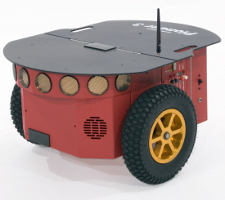
\includegraphics[width=0.4\textwidth]{pioneer.png}
   \caption*{Fonte: ROS (2019).}
   \label{fig:pioneer}
\end{figure}	


\subsection{Sensor de distância} 
O sensor de distância, é um tipo de sensor que mede a distância entre o robô e um objeto desejado.
Abaixo pode ser visto 16 feiches que representam as posições dos sensores de distância do Pioneer no Webots.

\begin{figure} [h!]	
   \centering
   \caption{Representação do sensor de distância}
   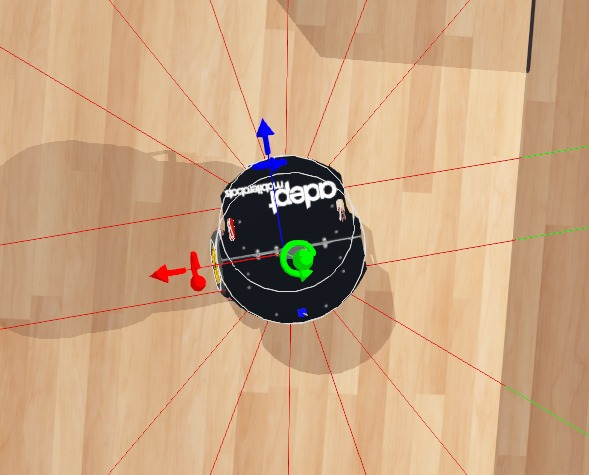
\includegraphics[width=0.4\textwidth]{sensord.png}
   \caption*{Fonte: Própria.}
   \label{fig:sensordistancia}

\end{figure}	

\subsection{Sensor de Luminosidade} 
A função do sensor é medir a intensidade de luz do ambiente ao seu redor, variando o estado de sua saída digital caso detectado um determinado nível de luminosidade. 
Abaixo pode ser visto um cubo azul que representa o sensor luminosidade adicionado no Pioneer.

\begin{figure} [h!]	
   \centering
   \caption{Representação do sensor de luminosidade}
   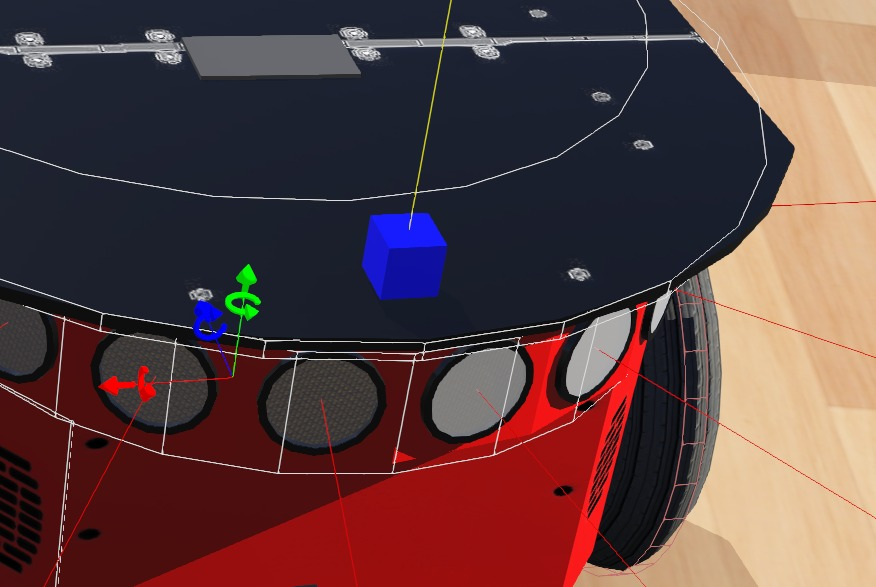
\includegraphics[width=0.4\textwidth]{sensorl.jpeg}
   \caption*{Fonte: Própria.}
   \label{fig:sensorluminosidade}
\end{figure}	

\section{Turtlesim}
\subsection{Nodes}
Um nó é apenas um arquivo executável dentro de um pacote do ROS. Nodes no ROS usam bibliotecas clientes para se comunicar com outros nós.
Nodes podem publicar e/ou subscrever em tópicos, além de poderem prover serviços também.\cite{WikiROS}
\subsection{Tópicos ROS}
Nodes podem publicar menssagens em tópicos assim como podem subescrever menssagens de tópicos.\cite{WikiROS}

Como é o exemplo dos nós turtlesim e turtle-teleop-key que se comuniçam entre si através do tópico turtle1command-velocity
turtle-teleop-key está publicando a tecla digitada no tópico, enquanto o turtlesim subescreve o mesmo tópico para receber a tecla digitada. \cite{WikiROS}

A imagem abaixo mostra os nós turtlesim e teleop, e o tópico command-velocity que faz a comunicação entre os dois nós.

\begin{figure} [h!]	
   \centering
   \caption{nós e tópicos ROS}
   
\includegraphics[width=0.5\textwidth]{net1.jpeg}
   \caption*{Fonte: Tutorials-UnderstandingTopics}
   \label{fig:nosetopicos}
\end{figure}	
\subsection{Publisher e Subscribers}

Publisher publica as informações ou mensagens no tópico e o subscriber subscreve o tópico e recebe as informações publicadas.\cite{WikiROS}

As mensagens são transmitidas em um tópico e cada tópico possui um nome exclusivo na rede ROS. Se um nó deseja compartilhar informações,
ele usa publisher para enviar dados a um tópico. Um nó que deseja receber essas informações usa subscriber desse mesmo tópico. \cite{WikiROS}

Além de seu nome exclusivo, cada tópico também possui um tipo de mensagem , que determina os tipos de mensagens que podem ser transmitidas naquele tópico.\cite{WikiROS}

O conceito de publisher e subscriber pode ser melhor visto na figura abaixo.
\begin{figure} [h!]	
   \centering
   \caption{publisher e subscriber ROS}
   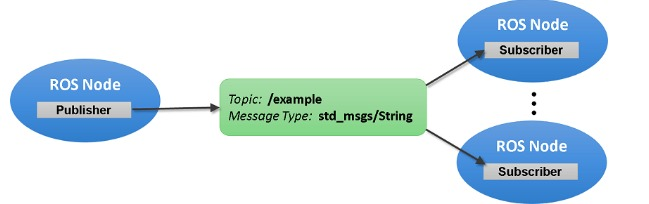
\includegraphics[width=0.5\textwidth]{sep.jpeg}
   \caption*{Fonte: la.mathworks.com/help//ros/ug/exchange-data-with-ros-publishers-and-subscribers.html}
   \label{fig:publisheresubscriber}
\end{figure}	

\subsection{Services e messages}
Os Nodes comunicam-se entre si publicando mensagens em tópicos . Uma mensagem é uma estrutura de dados simples, composta por campos digitados.\cite{WikiROS}

Os nodes também podem trocar uma mensagem de solicitação e resposta como parte de uma chamada de serviço ROS.

O modelo publisher e subscriber é um paradigma de comunicação muito flexível, mas seu transporte unilateral para muitos não é apropriado
para interações de solicitação e resposta RPC, que geralmente são necessárias em um sistema distribuído.\cite{WikiROS}

A solicitação e resposta é feita por meio de um Serviço, que é definido por um par de mensagens : Uma para a solicitação e outra para a resposta.
\begin{figure} [h!]	
   \centering
   \caption{services e messages ROS}
   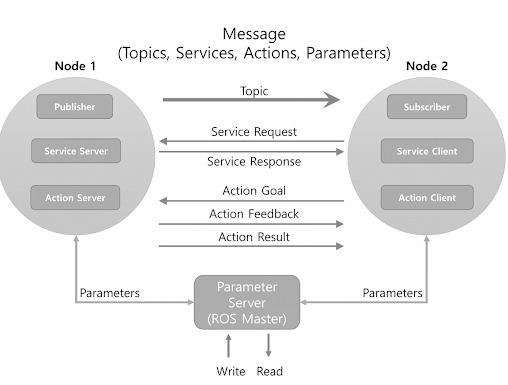
\includegraphics[width=0.4\textwidth]{sem.jpeg}
   \caption*{Fonte: robinrobotic.blogspot.com/2019/06/ros-terminology.html}
   \label{fig:servicesemessages}
\end{figure}	

 \section{Husky}
 %desenvolver mais
 \subsection{Move Base Demo}
 Realiza o planejamento autônomo básico e movimento no Husky com um scanner a laser publicando no tópico de digitalização.\cite{WikiROS}

 O nó move-base fornece uma interface ROS para configurar, executar e interagir com a pilha de navegação em um robô.
 \begin{figure} [h!]	
   \centering
   \caption{move base}
   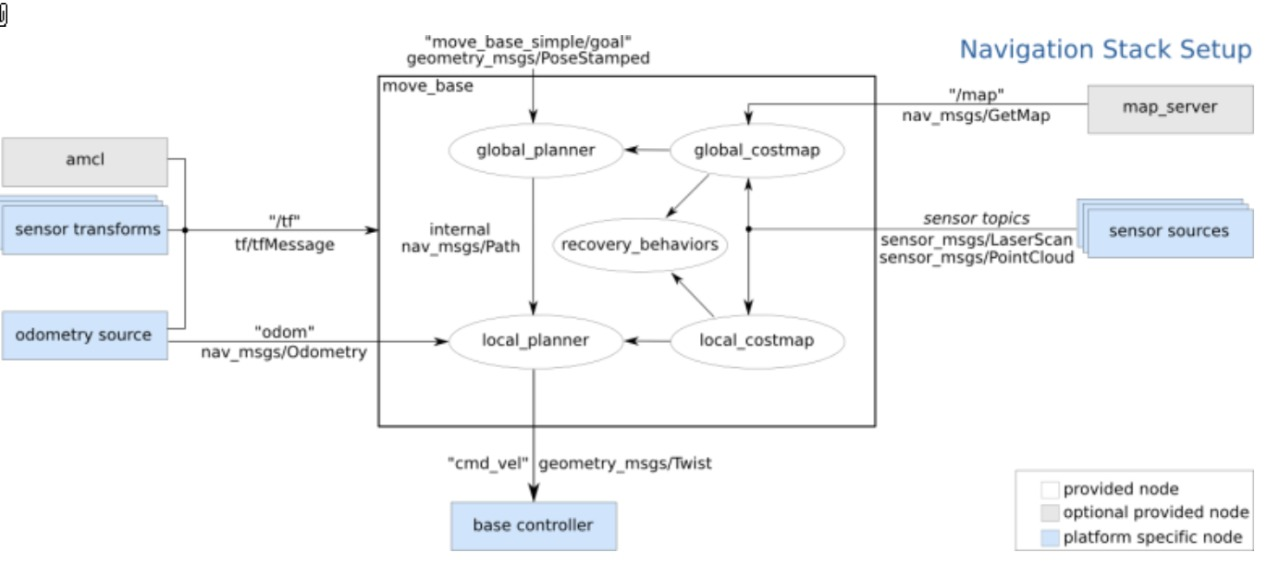
\includegraphics[width=0.5\textwidth]{mb.jpeg}
   \caption*{Fonte:}
   \label{fig:movebase}
\end{figure}

A pilha de navegação recebe informações de odometria e fluxos de sensores e emite comandos de velocidade para enviar ao robô.

Por padrão, o nó move-base executará as seguintes ações para tentar limpar o espaço:

Primeiro, os obstáculos fora de uma região especificada pelo usuário serão removidos do mapa do robô. Em seguida, se possível, o robô executará uma rotação no local para liberar espaço. Se isso também falhar, o robô limpará seu mapa de forma mais agressiva, removendo todos os obstáculos fora da região retangular na qual ele pode girar no lugar. Isso será seguido por outra rotação no local. Se tudo isso falhar, o robô considerará seu objetivo inviável e notificará o usuário de que ele foi abortado \cite{WikiROS}

\subsection{AMCL Demo}
Realiza o planejamento autônomo e movimento com localização em um Husky simulado com um scanner a laser publicando no tópico de digitalização.
amcl é um sistema de localização probabilística para um robô se movendo em 2D. Ele implementa a abordagem de localização adaptativa que usa um filtro de partículas para rastrear a posição de um robô em relação a um mapa conhecido. \cite{WikiROS}

\subsection{Gmapping}
realizar planejamento autônomo e movimento com localização e mapeamento simultâneo (SLAM), em um Husky simulado com um scanner a laser publicando no tópico de digitalização.
O pacote gmapping fornece SLAM baseado em laser, como um nó ROS chamado slam-gmapping. Usando slam-gmapping, você pode criar um mapa de grade de ocupação 2-D a partir de dados de laser e pose coletados por um robô móvel.\cite{WikiROS}

\subsection{Frontier Exploration}
Planejamento de exploração e gmapping para mapeamento e localização (SLAM).
Implementação de exploração de fronteira para ROS, estendendo-se na pilha de navegação existente. Ele aceita objetivos de exploração via actionlib, envia comandos de movimento para move-base.\cite{WikiROS}
 \section{CPP workbook}
 C++ é uma das linguagens mais usadas do mundo, uma das poucas linguagens de alto nível realmente compiladas e está em constante evolução.
 Esta linguagem tem serie de bibliotecas como a iostream que declara objetos que controlam a leitura e a gravação nos fluxos padrão. 
 \section{Python workbook 1 e 2}
 O Python traz características que possibilitam escrever o mesmo requisito em menos linhas de código que o necessário em outras linguagens de programação e hoje, além de adotado na construção de soluções web, também está sendo muito utilizado em aplicações que lidam com processamento de texto, machine learning e recomendação de conteúdo, áreas que não param de crescer.\cite{Python}
%----------------------------------------------------------

%--------- NEW SECTION ----------------------


%---------------picture------------------------------------
% \begin{figure}
%     \centering
%     \subfigure[Figure A]{\label{fig:a}\includegraphics[width=60mm]{./lq}}
%     \subfigure[Figure B]{\label{fig:b}\includegraphics[width=60mm]{./lq}}
%     \subfigure[Figure C]{\label{fig:c}\includegraphics[width=\textwidth]{./lq}}
%     \caption{Three simple graphs}
%     \label{fig:three graphs}
% \end{figure}
%----------------------------------------------------------

% \begin{figure}
%     \centering
%     \begin{subfigure}[b]{0.3\textwidth}
%         \centering
%         \includegraphics[width=\textwidth]{./lq}
%         \caption{$y=x$}
%         \label{fig:y equals x}
%     \end{subfigure}
%     \hfill
%     \begin{subfigure}[b]{0.3\textwidth}
%         \centering
%         \includegraphics[width=\textwidth]{./lq}
%         \caption{$y=3sinx$}
%         \label{fig:three sin x}
%     \end{subfigure}
%     \hfill
%     \begin{subfigure}[b]{0.3\textwidth}
%         \centering
%         \includegraphics[width=\textwidth]{./lq}
%         \caption{$y=5/x$}
%         \label{fig:five over x}
%     \end{subfigure}
%        \caption{Three simple graphs}
%        \label{fig:three graphs}
% \end{figure}


% %--------- NEW SECTION ----------------------
% \section{Assunto 2}
% \label{sec:ass2}
% flkjasdlkfjasdlkfjs

% \begin{table}[h]
%     \begin{subtable}[h]{0.45\textwidth}
%         \centering
%         \begin{tabular}{l | l | l}
%         Day & Max Temp & Min Temp \\
%         \hline \hline
%         Mon & 20 & 13\\
%         Tue & 22 & 14\\
%         Wed & 23 & 12\\
%         Thurs & 25 & 13\\
%         Fri & 18 & 7\\
%         Sat & 15 & 13\\
%         Sun & 20 & 13
%        \end{tabular}
%        \caption{First Week}
%        \label{tab:week1}
%     \end{subtable}
%     \hfill
%     \begin{subtable}[h]{0.45\textwidth}
%         \centering
%         \begin{tabular}{l | l | l}
%         Day & Max Temp & Min Temp \\
%         \hline \hline
%         Mon & 17 & 11\\
%         Tue & 16 & 10\\
%         Wed & 14 & 8\\
%         Thurs & 12 & 5\\
%         Fri & 15 & 7\\
%         Sat & 16 & 12\\
%         Sun & 15 & 9
%         \end{tabular}
%         \caption{Second Week}
%         \label{tab:week2}
%      \end{subtable}
%      \caption{Max and min temps recorded in the first two weeks of July}
%      \label{tab:temps}
% \end{table}
    \chapter{Desenvolvimento do projeto}
\label{chap:metod}
Nesta seção será descrito o procedimento utilizado para construção de cada um dos desafios.

\section{Webots}
O robô utilizado foi o Pionner o qual usa seus 16 sensores de distância pré-instalados para obter informações do mundo em todas as direções 
e um sensor adcional:o sensor de luminosidade que rastreia a irradiância local e envia um sinal para o robô quando ele lê mais de 750 W / m2, 
o que significa que está perto o suficiente da luminária de chão para disparar o STOP.

\subsection{controle}
A navegação do robô pelo mapa é baseada em uma máquina de 4 estados que determina se ele deve se mover para frente,
virar à esquerda, direita ou parar quando atingir seu objetivo final.

Assim, a divisão foi feita em quatro casos, são eles:
\begin{itemize}
    \item FORWARD: Anda para frente e se houver algum obstáculo à frente ele começa a tomar a decisão de virar em qualquer direção para evitá-lo.
    \item ESQUERDA: Vire à esquerda até que a detecção de objetos não seja mais possível;
    \item DIREITA: Vire à direita até que a detecção de objetos não seja mais possível;
    \item STOP: Quando o sensor de luz detecta a quantidade de luminosidade configurada (neste caso 750 W / m2), o robô deve parar.
\end{itemize}

\section{Turtlesim}

%desdobramento da função qualidade
\section{Husky}
\textit{Quality Function Deployment} é uma ferramenta de qualidade que auxilia na conversão das demandas do cliente em características de qualidade do produto. Dessa forma, no primeiro ciclo do QFD foram analisados os requisistos do cliente e os requisitos técnicos necessários, sinalizando os pontos mais importantes e as relações entre estes. O resultado foi exposto na \ref{fig:QFD}

\begin{figure} [h!]	
    \centering
    \caption{ Primeiro ciclo QFD}
    \includegraphics[width=0.8\textwidth]{Figures/QFD}
    \caption*{Fonte: Autoria própria.}
    \label{fig:QFD}
\end{figure}
 Através do QFD foi possível observar 

% %--------- NEW SECTION ----------------------
% \section{Interface do Usuário}
% \label{sec:ui}
% \lipsum[1]

% %--------- NEW SECTION ----------------------
% \section{Simulação do sistema}
% \label{sec:sim}
% \lipsum[2-4]


    \chapter{Resultados.}
\label{chap:result}
Os resultados obtidos nos desafios foram:
%--------- NEW SECTION ----------------------
\section{Webots}

Cada um dos 16 sensores de distância incluídos no Pionner são encontrados no arquivo de controle do robô challengecontroller.c
e contêm valores de peso para cada roda, que são baseados na posição do sensor no robô e mostram como sua leitura influencia o 
comportamento do duas rodas. Além disso, o valor do peso auxilia na tomada de decisão, pois, se a leitura de algum sensor cair 
abaixo do valor mínimo definido, significa que o robô está próximo a um obstáculo e deve mudar de direção usando um dos casos acima. 
No final, ele foi usado para determinar o comportamento do robô em todos os valores de peso em cada roda vezes um fator de velocidade, 
que é dependente tanto da relação de leitura do sensor quanto do valor de distância mínima.

Também faz parte do controle o sensor de luz que foi adicionado para completar o desafio, 
este sensor ativa o estado STOP quando detecta um brilho maior que 750 W / m2 e assim o desafio é concluído.

As fotos mostram o pioneer iniciando, chegando na área luminosa e parando no tempo correto, completando assim o desafio proposto,
para uma melhor visualização da solução tem um link do video logo abaixo e o controle pode ser encontrado no repositório https://github.com/marcellabecker/desafiorobotica 

\begin{figure} [h!]	
    \centering
    \caption{Pioneer iniciando o percurso}
    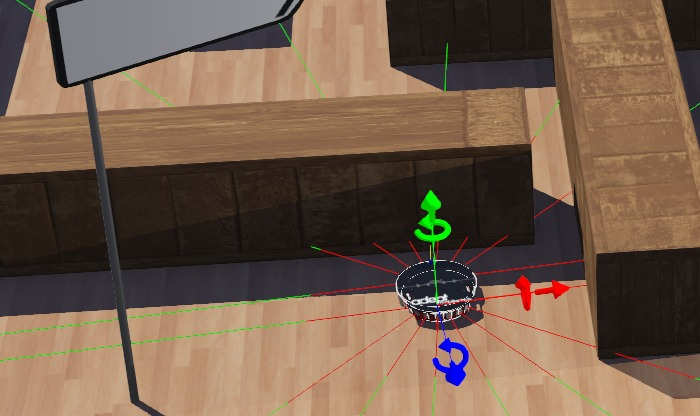
\includegraphics[width=0.5\textwidth]{inicio.jpeg}
    \caption*{Fonte:Própria.}
    \label{fig:inciodopercurso}
\end{figure}

\begin{figure} [h!]	
    \centering
    \caption{Pioneer completando o percurso}
    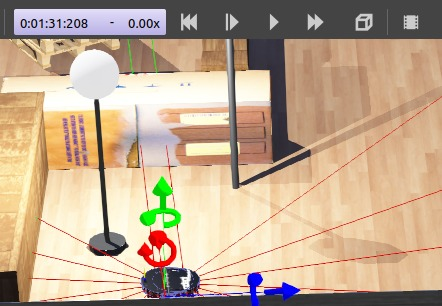
\includegraphics[width=0.5\textwidth]{fim.jpeg}
    \caption*{Fonte:Própria.}
    \label{fig:fimdopercurso}
\end{figure}



Link para assistir ao vídeo:https://www.youtube.com/watch?v=RftRevxZUOE

\section{Turtlesim SETPOINT}
Inicialmente no codigo foi feita uma função de callback que é chamada quando o subscriber recebe um dado do tópico. 
Logo depois o nó é iniciado, para que possa ser feito os publishers e subscribers no tópicos, sendo assim 
vel-publisher publica mensagens no tópico cmd-vel e posecb recebe a msg de coodenada da posição.

Goal-x e goal-y recebem os inputs das coordenadas x e y para onde a tartaruga deve ir. 

kp-lin e kp-ang são os controles de velocidade linear e angular definidos para que a tartaruga nao ande muito rapido nem
muito devagar e controla o seu angulo de curvatura durante o movimento.

A FUNÇÃO is-shutdown() verifica se seu programa deve sair, portanto enquanto não entrar no if que está dentro do while significa que o erro ainda é 
maior que 0.1 e a turtle ainda não chegou ao seu destino sendo assim o programa deve continuar rodando, ate que o o erro seja 0.1 como manda o desafio
e ela deve parar.

As figuras abaixos mostram a janela da turtle antes da coordenadas e depois dela andar para coordenada (1,1).

\begin{figure} [h!]	
    \centering
    \caption{janela da turtle}
    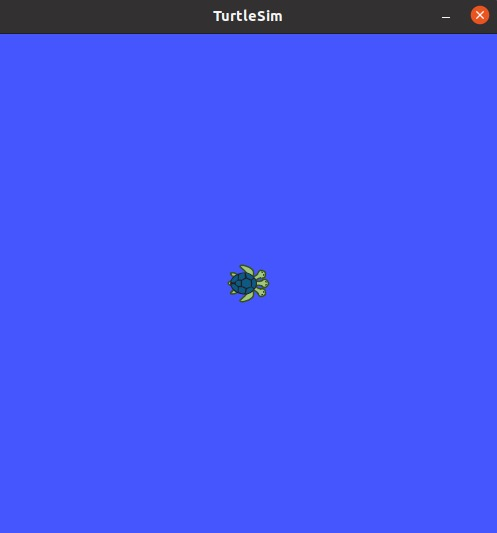
\includegraphics[width=0.35\textwidth]{antes.jpeg}
    \caption*{Fonte:Própria.}
    \label{fig:inicio}
\end{figure}

\begin{figure} [h!]	
    \centering
    \caption{Turtle chegou ao destino}
    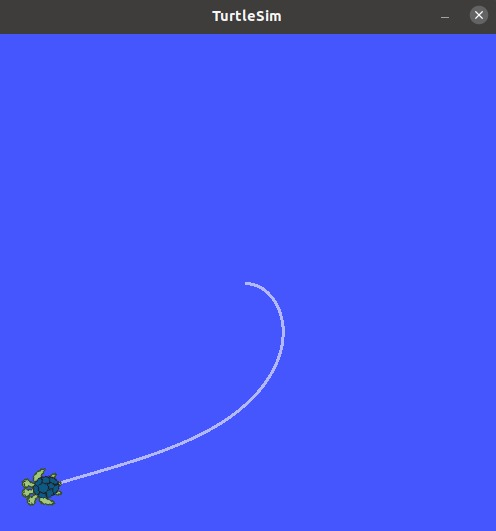
\includegraphics[width=0.35\textwidth]{depois.jpeg}
    \caption*{Fonte:Própria.}
    \label{fig:fim}
\end{figure}
Para uma melhor visualização da solução tem um link do video 
logo abaixo e o controle pode ser encontrado no repositório https://github.com/marcellabecker/turtle  

Link para assistir ao vídeo:https://youtu.be/NNkwSgDScuY
\section{Husky}
\subsection{Move-base}
Com todos os comando de movimentação já configurados e as janelas rviz e gazebo ja abertas a movimentação é feita pelo mouse podendo também usar o teclado pelo comando teleop-twist-keyboard ou por controle remoto.
As imagens abaixo mostram antes, durante e depois que a movimentação for concluida. 

\begin{figure} [h!]	
    \centering
    \caption{Husky antes do movimento}
    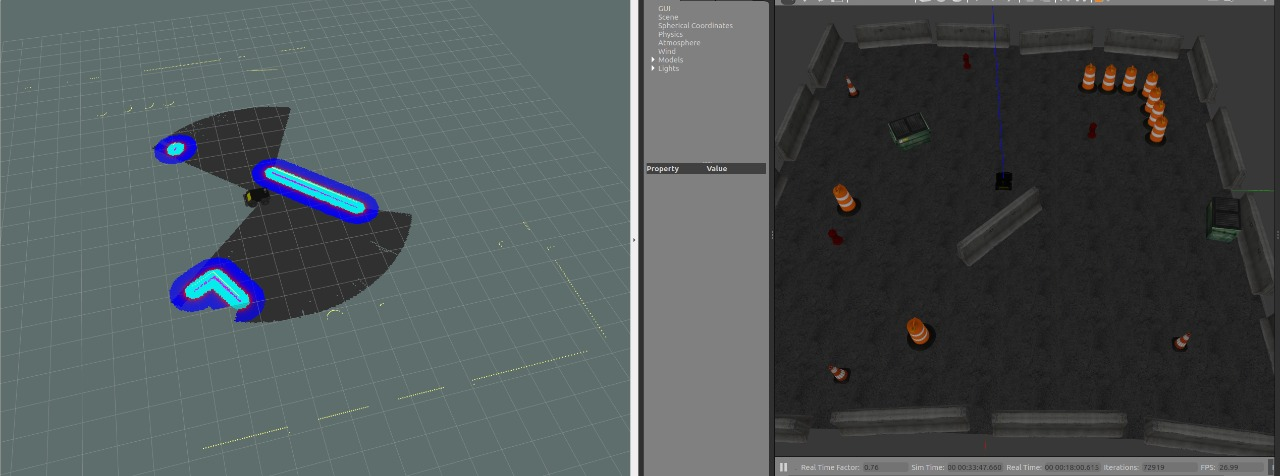
\includegraphics[width=0.7\textwidth]{antesmb.jpeg}
    \caption*{Fonte:Própria.}
    \label{fig:antesmovebase}
\end{figure}
\begin{figure} [h!]	
    \centering
    \caption{Husky durante o movimento}
    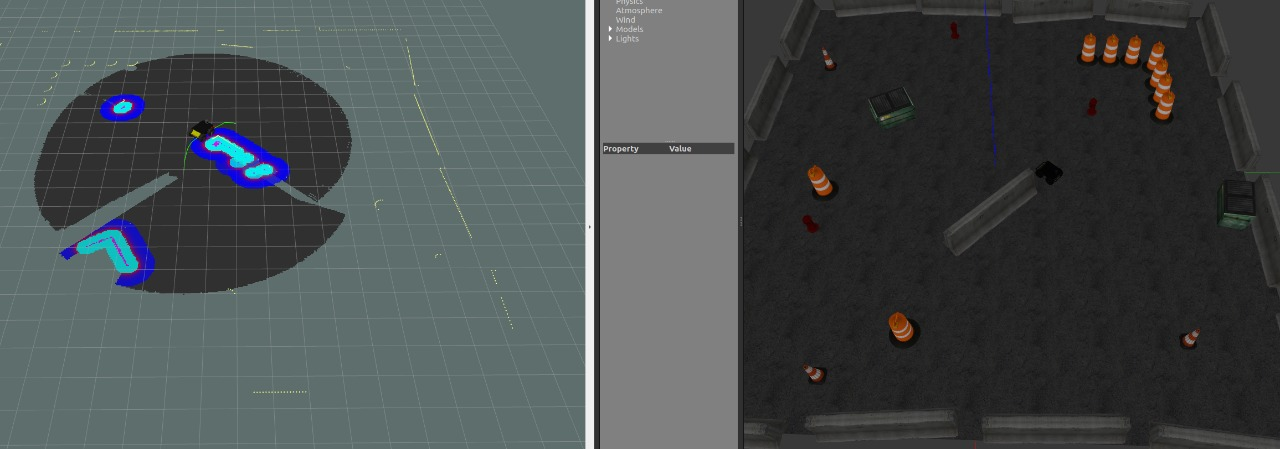
\includegraphics[width=0.7\textwidth]{durantemb.jpeg}
    \caption*{Fonte:Própria.}
    \label{fig:durantemovebase}
\end{figure}
\begin{figure} [h!]	
    \centering
    \caption{Husky depois o movimento}
    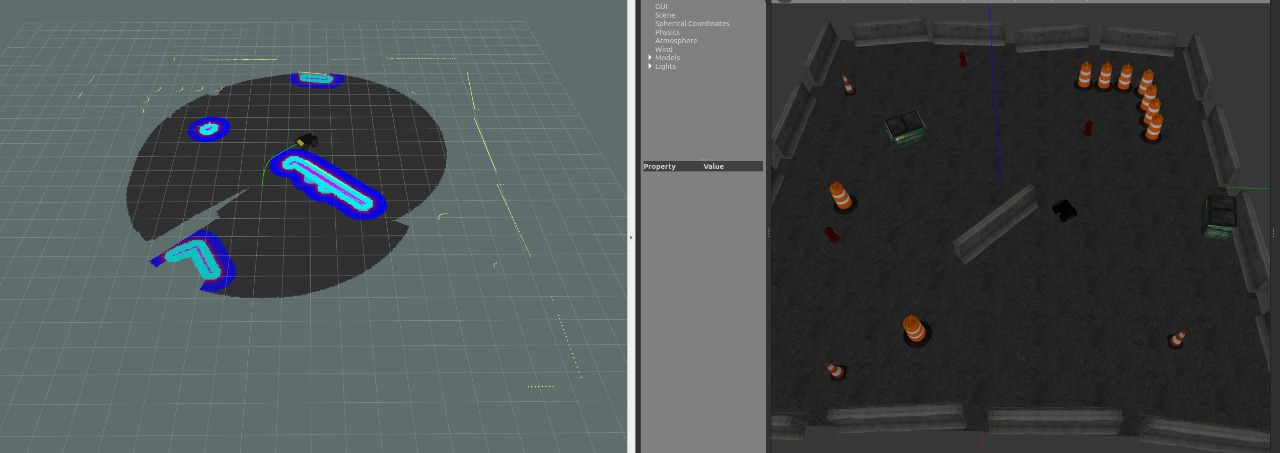
\includegraphics[width=0.7\textwidth]{depoismb.jpeg}
    \caption*{Fonte:Própria.}
    \label{fig:depoismovebase}
\end{figure}
\subsection{AMCL}
Com todos os comando de movimentação já configurados e as janelas rviz e gazebo ja abertas a movimentação é feita pelo mouse podendo também usar o teclado pelo comando teleop-twist-keyboard ou por controle remoto.
As imagens abaixo mostram antes, durante e depois que a movimentação for concluida.
\begin{figure} [h!]	
    \centering
    \caption{Husky antes do movimento}
    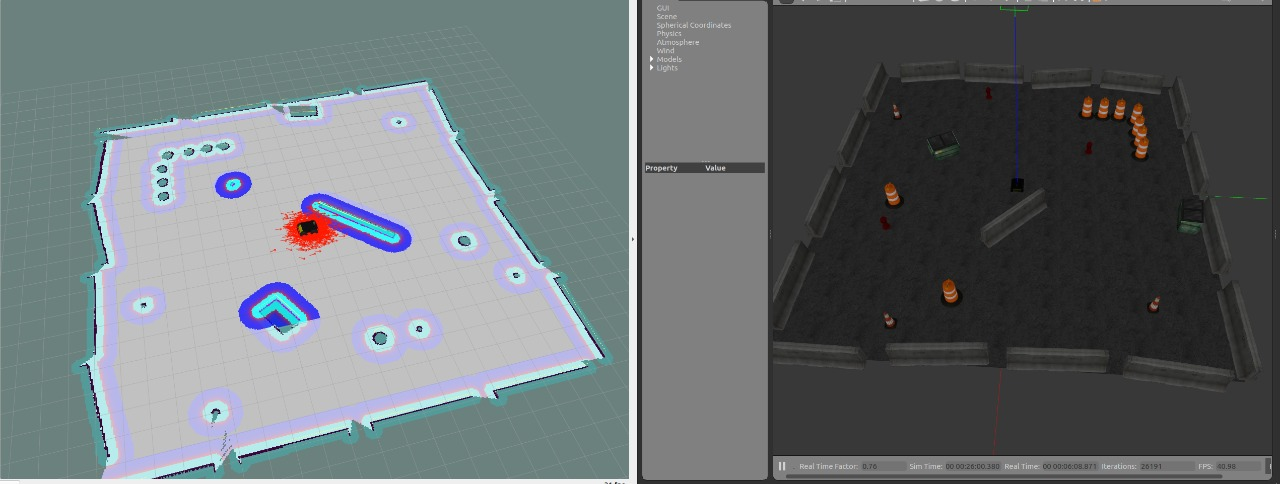
\includegraphics[width=0.7\textwidth]{antesamcl.jpeg}
    \caption*{Fonte:Própria.}
    \label{fig:antesamcl}
\end{figure}
\begin{figure} [h!]	
    \centering
    \caption{Husky durante o movimento}
    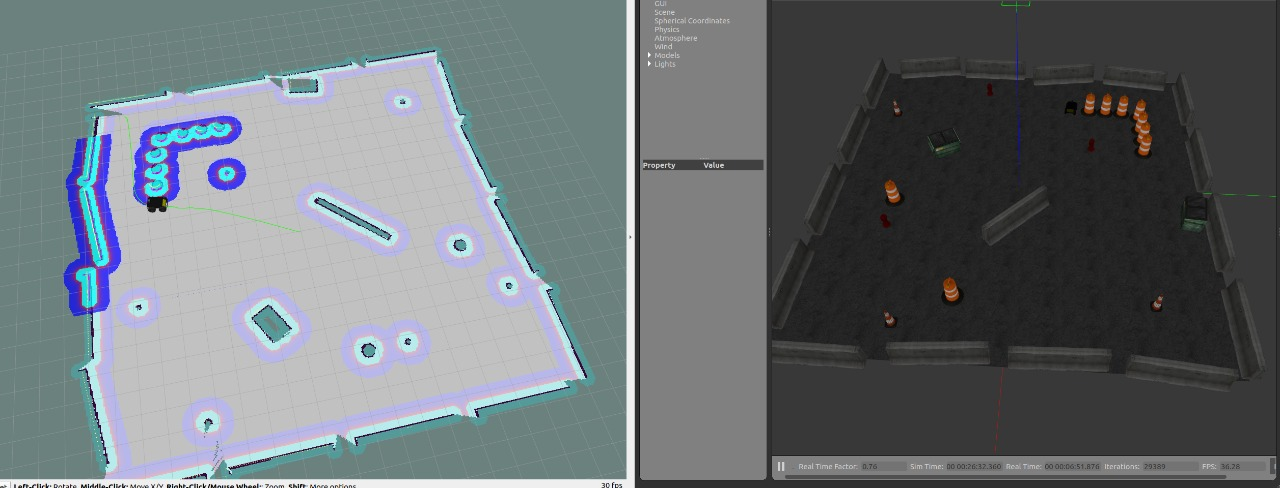
\includegraphics[width=0.7\textwidth]{duranteamcl.jpeg}
    \caption*{Fonte:Própria.}
    \label{fig:duranteamcl}
\end{figure}
\begin{figure} [h!]	
    \centering
    \caption{Husky depois o movimento}
    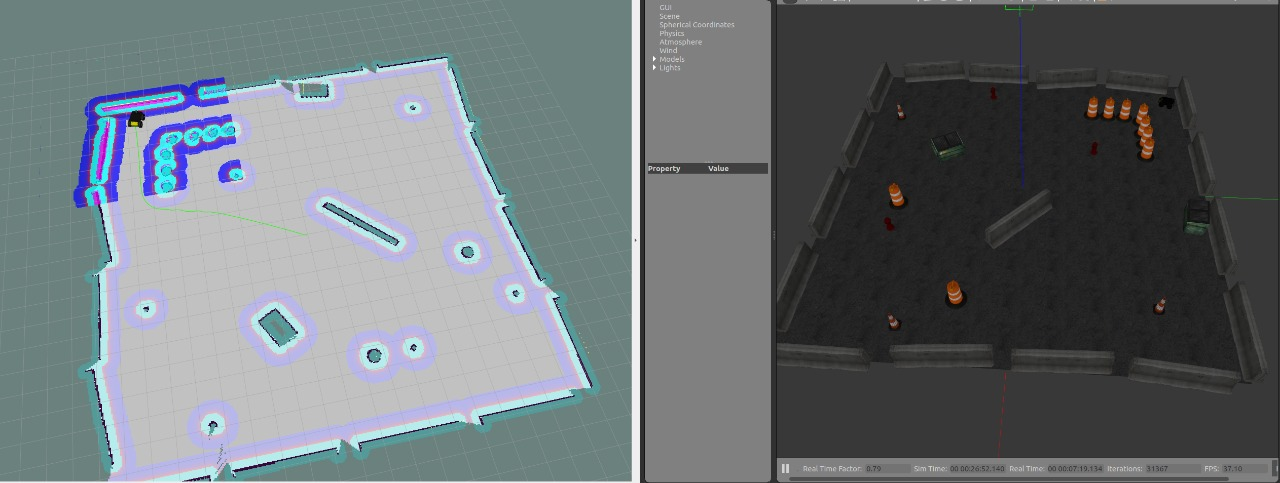
\includegraphics[width=0.7\textwidth]{depoisamcl.jpeg}
    \caption*{Fonte:Própria.}
    \label{fig:depoisamcl}
\end{figure}
É possivel ver que diferente do move-base o Husky consegue ter um alcance bem maior de visualização, o todos formados pelo mapa e o laiser destaca os que estão mais perto.
\subsection{Gmapping}
Com todos os comando de movimentação já configurados e as janelas rviz e gazebo ja abertas a movimentação é feita pelo mouse podendo também usar o teclado pelo comando teleop-twist-keyboard ou por controle remoto.

As imagens abaixo mostram antes, durante e depois que a movimentação for concluida.
\begin{figure} [h!]	
    \centering
    \caption{Husky antes do movimento}
    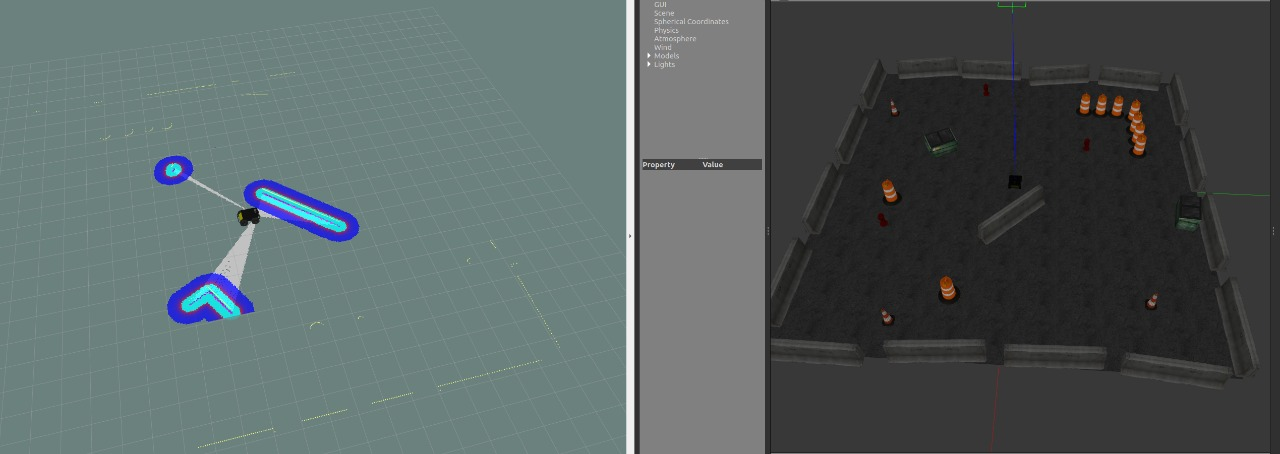
\includegraphics[width=0.7\textwidth]{antesgm.jpeg}
    \caption*{Fonte:Própria.}
    \label{fig:antesgmappinng}
\end{figure}
\begin{figure} [h!]	
    \centering
    \caption{Husky durante o movimento}
    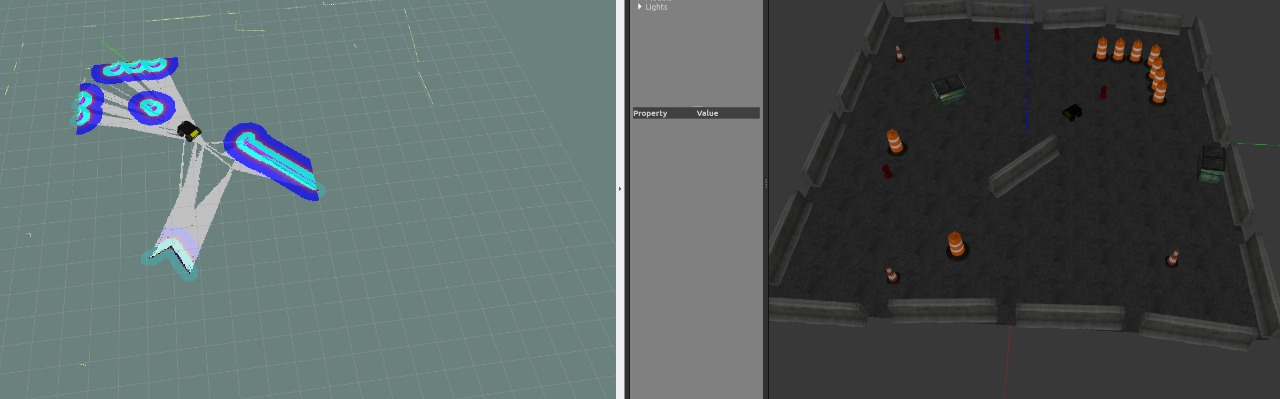
\includegraphics[width=0.7\textwidth]{durantegm.jpeg}
    \caption*{Fonte:Própria.}
    \label{fig:durantegmapping}
\end{figure}
\begin{figure} [h!]	
    \centering
    \caption{Husky depois o movimento}
    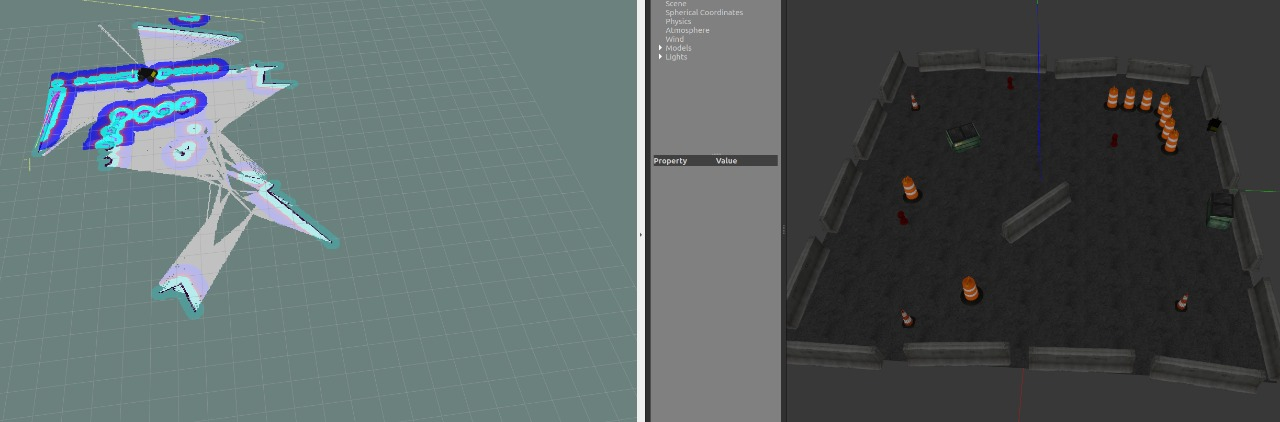
\includegraphics[width=0.7\textwidth]{depoisgm.jpeg}
    \caption*{Fonte:Própria.}
    \label{fig:depoisgmapping}
\end{figure}



A diferença do Gmapping é o SLAM que localiza e mapeia o ambiente simultâneamente, como pode ser visto o Husky enquando está se localizando para andar no mapa, também constrói o mapa.
\subsection{Frontier-exploration}
Com todos os comando de movimentação já configurados e as janelas rviz e gazebo ja abertas a movimentação é feita pelo mouse podendo também usar o teclado pelo comando teleop-twist-keyboard ou por controle remoto.

As imagens abaixo mostram antes, durante e depois que a movimentação for concluida.
\begin{figure} [h!]	
    \centering
    \caption{Husky antes do movimento}
    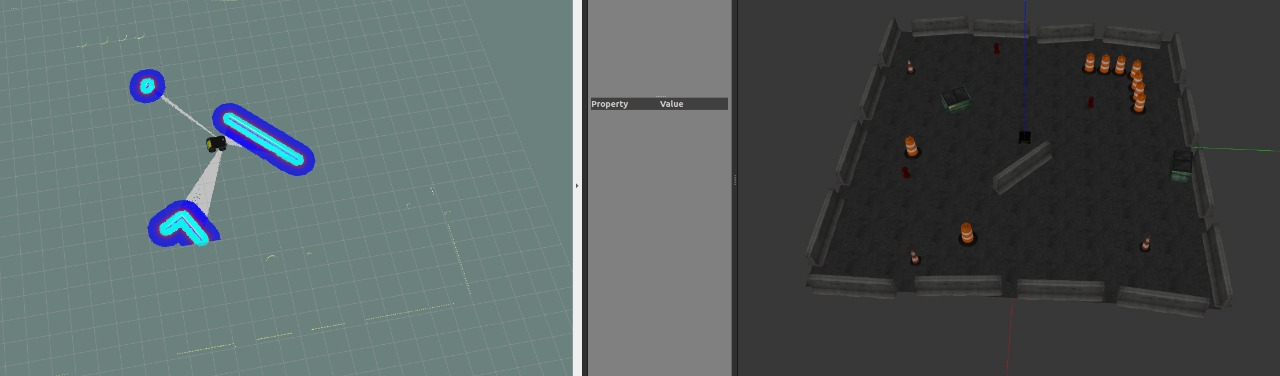
\includegraphics[width=0.7\textwidth]{antesf.jpeg}
    \caption*{Fonte:Própria.}
    \label{fig:antesFrontier-exploration}
\end{figure}
\begin{figure} [h!]	
    \centering
    \caption{Husky durante o movimento}
    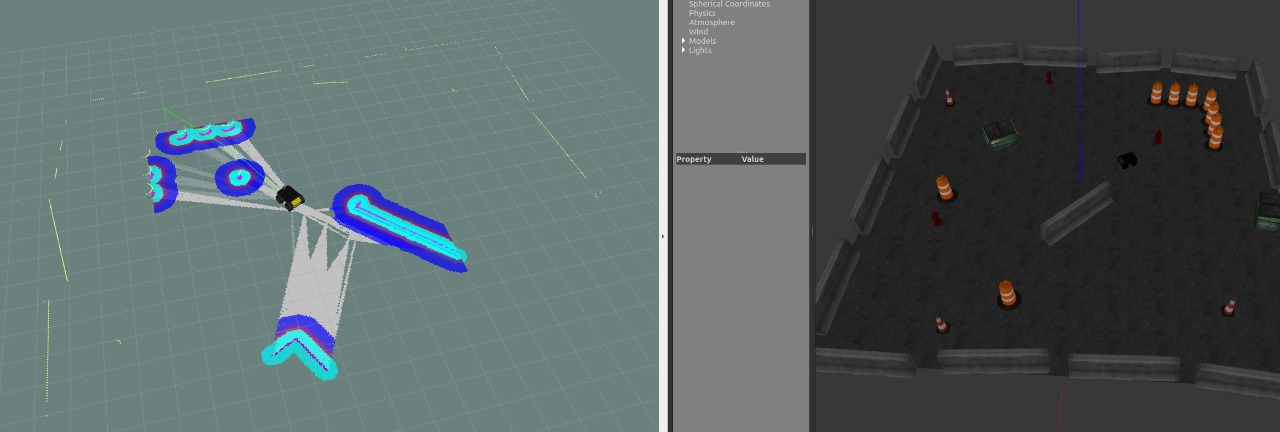
\includegraphics[width=0.7\textwidth]{durantef.jpeg}
    \caption*{Fonte:Própria.}
    \label{fig:duranteFrontier-exploration}
\end{figure}
\begin{figure} [h!]	
    \centering
    \caption{Husky depois o movimento}
    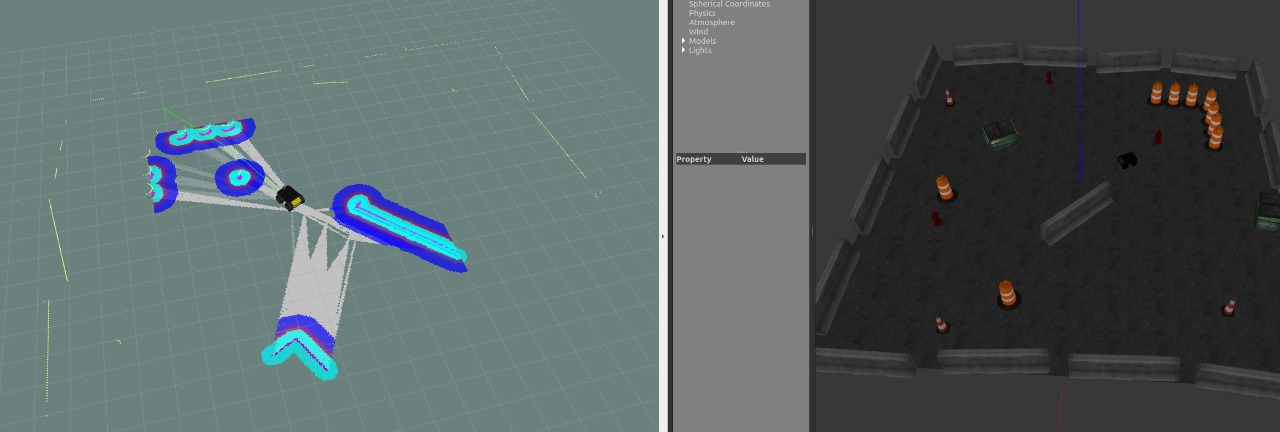
\includegraphics[width=0.7\textwidth]{depoisf.jpeg}
    \caption*{Fonte:Própria.}
    \label{fig:depoisFrontier-exploration}
\end{figure}

Conforme o robô se move, você deve ver o mapa estático cinza crescer. Ocasionalmente, o algoritmo de gmapping irá realocar o robô, causando um salto discreto no mapa. Quando a meta de exploração for concluída, você verá uma mensagem escrito DONE na janela do terminal.
\section{cpp}
-Desafio do Triângulo de Pascal:
Para demonstrar os resultados obtidos foi compilado o codigo, a figura a baixo mostra o resultado da linha 4 do triangulo.
\begin{figure} [h!]	
    \centering
    \caption{triangulo ate linha 4}
    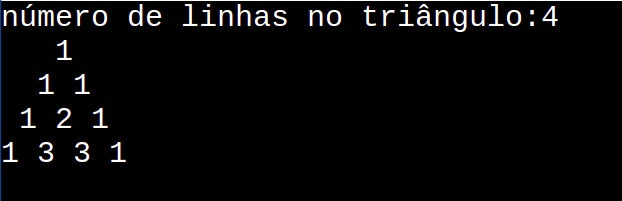
\includegraphics[width=0.7\textwidth]{rt.jpeg}
    \caption*{Fonte:Própria.}
    \label{fig:triangulodepascal}
\end{figure}

- Permutação de cordas:
Após o codigo ser bildado foi colocado a palavra tia como no exemplo do PDF dado, na figura a baixo mostra o resultado.
\begin{figure} [h!]	
    \centering
    \caption{Permutação da palavra tia}
    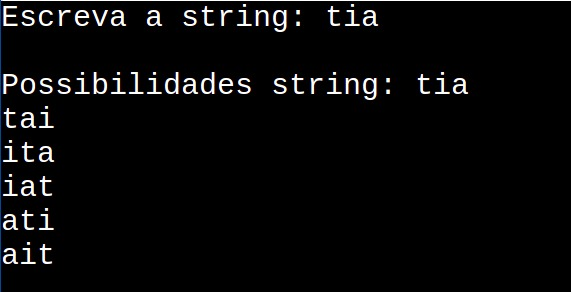
\includegraphics[width=0.5\textwidth]{rp.jpeg}
    \caption*{Fonte:Própria.}
    \label{fig:permutacao}
\end{figure}
- Autoimpressão:
%\begin{figure} [h!]	
%    \centering
%    \caption{Permutação da palavra tia}
%    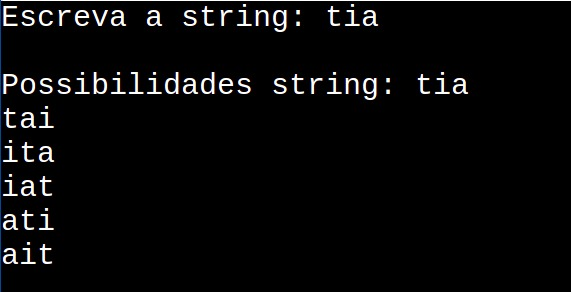
\includegraphics[width=0.7\textwidth]{rp.jpeg}
%    \caption*{Fonte:Própria.}
%    \label{fig:permutacao}
%\end{figure}

\section{Python 1}
-Mediana de Três Valores:
Após colocar os 3 números foi o programa cálculou a médiada dos 3 através da formula.

Como pode ser visto na figura abaixo:
\begin{figure} [h!]	
    \centering
    \caption{Mediana}
    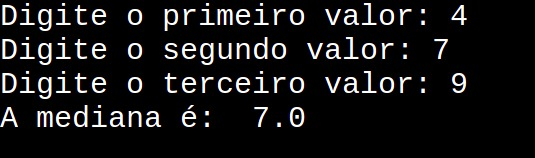
\includegraphics[width=0.8\textwidth]{mediana1.jpeg}
    \caption*{Fonte:Própria.}
    \label{fig:med}
\end{figure}

-Os Doze Dias do Natal:
Nesse desafio foi feita a plotagem completa da musica The twelve Days of christmas.

O resultado pode ser visualizado na imagem:
\begin{figure} [h!]	
    \centering
    \caption{Musica}
    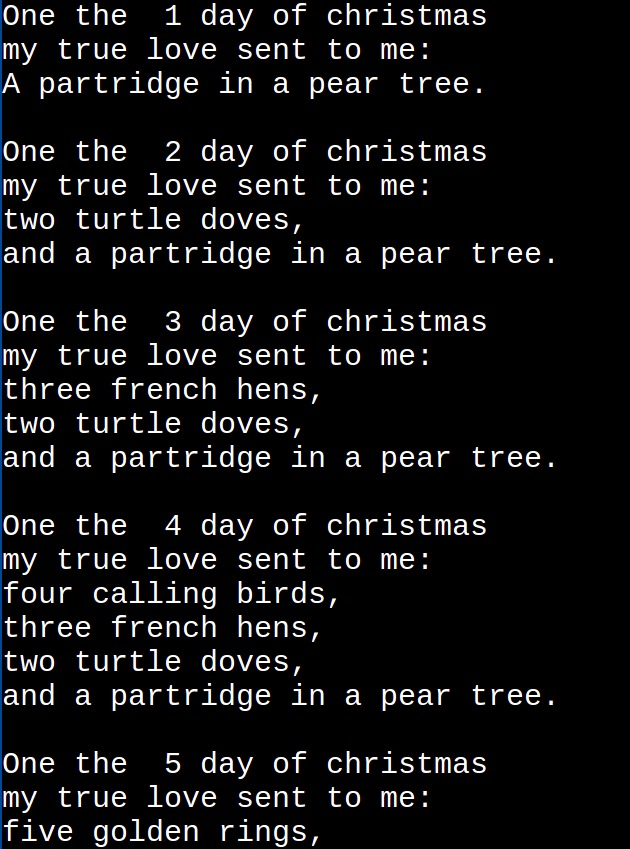
\includegraphics[width=0.8\textwidth]{12.jpeg}
    \caption*{Fonte:Própria.}
    \label{fig:musica}
\end{figure}



-Centralize uma corda no terminal:

Nesse desafio aṕos a escolha da palavra centralização e dos espados de 25 foi plotada de forma certralizada ao terminal de 25 espaços vazios.
O resultado pode ser visualizado na imagem:
\begin{figure} [h!]	
    \centering
    \caption{centralização}
    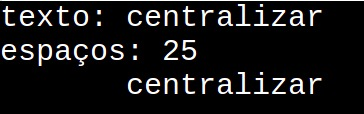
\includegraphics[width=0.9\textwidth]{central.jpeg}
    \caption*{Fonte:Própria.}
    \label{fig:centralizar}
\end{figure}






-Capitalize-o:

Nesse desafio foi posto uma frase começando com letra minuscula e um nome após os ; também minusculos e foi corrigido.
O resultado pode ser visualizado na imagem:
\begin{figure} [h!]	
    \centering
    \caption{Maiúsculo e minúsculo}
    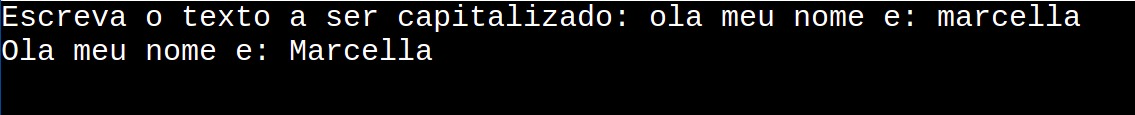
\includegraphics[width=0.7\textwidth]{cap.jpeg}
    \caption*{Fonte:Própria.}
    \label{fig:cap}
\end{figure}
    \chapter{Conclusão}
\label{chap:conc}

Ao final de todos os desafios foi possivel ver o grande diferencial na carreira profissional para quem seguir a área da robótica.
Sendo assim todos os desafios chegaram ao seu objetivo final proposto com exito, podendo ser encontrados com mais detalhes no github: https://github.com/marcellabecker?tab=repositories.


%\section{Considerações finais}
%\label{sec:consid}

%Brevemente comentada no texto acima, nesta se\c{c}\~ao o
%pesquisador (i.e. autor principal do trabalho cient\'ifico) deve
%apresentar sua opini\~ao com respeito \`a pesquisa e suas
%implica\c{c}\~oes. Descrever os impactos (i.e.
%tecnol\'ogicos,sociais, econ\^omicos, culturais, ambientais,
%políticos, etc.) que a pesquisa causa. N\~ao se recomenda citar
%outros autores.


    % include more chapters ...
%
% ----------------------------------------------------------------------------
% Include thesis appendices
    \begin{thesisappendices}
        % Thesis Appendix -------------------------------------------------------

%\chapter{Diagramas mecânicos}
%\label{Append:diagmec}



        % Thesis Appendix -------------------------------------------------------

%\chapter{Diagramas eletro-eletrônicos}
%\label{Append:diagele}



        % Thesis Appendix -------------------------------------------------------

%\chapter{Logbook}
%\label{Append:log}



    \end{thesisappendices}
%
% ----------------------------------------------------------------------------
% Configurar as referencias bibliograficas
	\renewcommand\bibname{Referências}
    \addcontentsline{toc}{chapter}{Referências}
    \bibliography{References/referencias}
%
% ----------------------------------------------------------------------------
% Finishing him
    \include{Others/ultimafolha}
\end{document}
%
% -------------------------------------------------------------------------------
% Aqui termina a formatação para o documento.
% In God We Trust. All Other Bring Data. 
%
% -------------------------------------------------------------------------------